\documentclass{beamer}
\usepackage{graphicx}
\usepackage{xcolor}
\usepackage{tikz}
\usepackage{amsmath}

\definecolor{purpleblue}{RGB}{80, 80, 180}
\definecolor{novelPurple}{RGB}{98, 54, 255}
\definecolor{softPurple}{RGB}{180, 170, 255}
\definecolor{softGray}{RGB}{235, 235, 245}
\definecolor{lightText}{RGB}{90, 90, 110}

\usetheme{Madrid}
\usecolortheme{dolphin}
\graphicspath{{static/course_materials/}{static/hard/}{./}}

\setbeamerfont{title}{size=\Large,series=\bfseries}
\setbeamerfont{frametitle}{size=\LARGE,series=\bfseries}
\setbeamercolor{frametitle}{fg=white, bg=novelPurple}
\setbeamercolor{title}{fg=white, bg=purpleblue}

\title[SAT Hard Question 10]{\textbf{SAT Hard Question\\ Set 10}}
\author{\textbf{Jack Zeng}}
\institute{\textcolor{white}{\textbf{Novel Prep}}}
\date{\today}

\begin{document}

\begin{frame}
    \titlepage
    \vfill
    \begin{flushright}
        \textcolor{purpleblue}{\Huge \textbf{Novel Prep}}
    \end{flushright}
\end{frame}

\begin{frame}
    \begin{tikzpicture}[remember picture, overlay]
        \shade[top color=softPurple, bottom color=softGray]
            (current page.north west) rectangle (current page.south east);
        \node[align=center] at (current page.center) {
            {\Huge\bfseries\textcolor{purpleblue}{Novel Prep}} \\[0.5cm]
            {\Large\itshape\textcolor{lightText}{Phase 2 · Hard Question Practice}}
        };
    \end{tikzpicture}
\end{frame}

\begin{frame}{Overview}
    \tableofcontents
\end{frame}

\begin{frame}
\section{Hard Question Set 10}
    \begin{tikzpicture}[remember picture, overlay]
        \shade[top color=softPurple, bottom color=softGray]
            (current page.north west) rectangle (current page.south east);
        \node[align=center] at (current page.center) {
            {\LARGE\bfseries\textcolor{purpleblue}{Hard Question Set 10}} \\[0.5cm]
            {\Large\itshape\textcolor{lightText}{8 SAT-style challenge problems}}
        };
    \end{tikzpicture}
\end{frame}

% --- Question 1 ---
\begin{frame}{Question 1}
\small
\begin{center}
    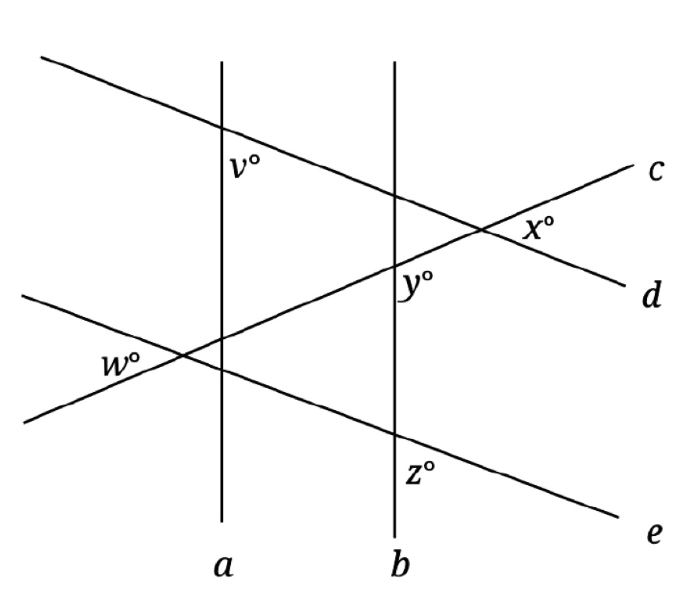
\includegraphics[width=0.42\linewidth]{hard_10_f8.png}
\end{center}

In the figure, parallel lines \(a\) and \(b\) are intersected by lines \(c\), \(d\), and \(e\).

If \(z = 49^\circ\), \(y = 136^\circ\), and \(v < z\), which statement about \(x\) and \(w\) must be true?
\vspace{0.35cm}
\begin{enumerate}
    \item[A.] \(x < w\)
    \item[B.] \(x > w\)
    \item[C.] \(x = w\)
    \item[D.] \(x + w = 90\)
\end{enumerate}
\end{frame}
\begin{frame}{Answer 1}
\small
\textbf{Correct Answer:} B
\end{frame}

% --- Question 2 ---
\begin{frame}{Question 2}
\small
The functions \(f\) and \(g\) are defined by the given equations below, where \(x \geq 0\).

Which of the following equations displays, as a constant or coefficient, the minimum value of the function it defines?

\begin{itemize}
\item[I.] \(f(x) = 16(1.3)^{x+5}\)
\item[II.] \(g(x) = 16(1.09)(1.3)^{x+3}\)
\end{itemize}
\vspace{0.35cm}
\begin{enumerate}
    \item[A.] I only
    \item[B.] II only
    \item[C.] I and II
    \item[D.] Neither I nor II
\end{enumerate}
\end{frame}
\begin{frame}{Answer 2}
\small
\textbf{Correct Answer:} D
\end{frame}

% --- Question 3 ---
\begin{frame}{Question 3}
\small
The table shows values of \(x\) and corresponding values of \(g(x)\), where:
\[
g(x) = \frac{f(x)}{x + 3}
\]
and \(f(x)\) is a linear function.

What is the \(y\)-intercept of the graph of \(y = f(x)\) in the \(xy\)-plane?

\[
\begin{array}{c|c}
x & g(x) \\
\hline
-15 & 3 \\
-6 & 0 \\
9 & 5 \\
\end{array}
\]
\vspace{0.35cm}
\begin{enumerate}
    \item[A.] \((0, -6)\)
    \item[B.] \((0, 4)\)
    \item[C.] \((0, 8)\)
    \item[D.] \((0, 24)\)
\end{enumerate}
\end{frame}
\begin{frame}{Answer 3}
\small
\textbf{Correct Answer:} D
\end{frame}

% --- Question 4 ---
\begin{frame}{Question 4}
\small
The positive number \(a\) is 2,106\% of the sum of the positive numbers \(b\) and \(c\), and \(b\) is 81\% of \(c\).

What percent of \(b\) is \(a\)?
\vspace{0.35cm}
\begin{enumerate}
    \item[A.] 4,706\%
    \item[B.] 2,600\%
    \item[C.] 38.12\%
    \item[D.] 21.87\%
\end{enumerate}
\end{frame}
\begin{frame}{Answer 4}
\small
\textbf{Correct Answer:} A
\end{frame}

% --- Question 5 ---
\begin{frame}{Question 5}
\small
In the given equation, \(u\) is a positive constant.

The sum of the solutions to the equation is 1. What is the value of \(u\)?
\[
7x^2(3x - 11)(3x - u) = 0
\]
\vspace{0.35cm}
\begin{enumerate}
    \item[A.] 1
    \item[B.] -8
    \item[C.] \(\frac{11}{3}\)
    \item[D.] \(\frac{8}{3}\)
\end{enumerate}
\end{frame}
\begin{frame}{Answer 5}
\small
\textbf{Correct Answer:} B
\end{frame}

% --- Question 6 ---
\begin{frame}{Question 6}
\small
Which of the following values of \(x\) satisfy the equation
\[
-3x^2 + 12x + 4 = 0
\]
\vspace{0.35cm}
\begin{enumerate}
    \item[A.] 0
    \item[B.] \(-2\) and 2
    \item[C.] \(2 - \frac{2\sqrt{6}}{3}\) and \(2 + \frac{2\sqrt{6}}{3}\)
    \item[D.] \(2 - \frac{4\sqrt{3}}{3}\) and \(2 + \frac{4\sqrt{3}}{3}\)
\end{enumerate}
\end{frame}
\begin{frame}{Answer 6}
\small
\textbf{Correct Answer:} D
\end{frame}

% --- Question 7 ---
\begin{frame}{Question 7}
\small
A line intersects two parallel lines, forming four acute angles and four obtuse angles.

The measure of one of these eight angles is \((7x - 250)^\circ\).

The sum of the measures of four of the eight angles is \(k\).

Which of the following could **not** be equivalent to \(k\) for all values of \(x\)?
\vspace{0.35cm}
\begin{enumerate}
    \item[A.] \(-14x + 1540\)
    \item[B.] \(14x - 320\)
    \item[C.] \(-28x + 1720\)
    \item[D.] 360
\end{enumerate}
\end{frame}
\begin{frame}{Answer 7}
\small
\textbf{Correct Answer:} A
\end{frame}

% --- Question 8 ---
\begin{frame}{Question 8}
\small
The triangle inequality theorem states that the sum of any two sides of a triangle must be greater than the length of the third side.

If a triangle has side lengths of 7 and 10, which inequality represents the possible lengths, \(x\), of the third side of the triangle?
\vspace{0.35cm}
\begin{enumerate}
    \item[A.] \(x < 17\)
    \item[B.] \(x > 17\)
    \item[C.] \(3 < x < 17\)
    \item[D.] \(x < 3\) or \(x > 17\)
\end{enumerate}
\end{frame}
\begin{frame}{Answer 8}
\small
\textbf{Correct Answer:} C
\end{frame}

\begin{frame}{}
    \begin{tikzpicture}[remember picture, overlay]
        \shade[top color=novelPurple!40, bottom color=white]
            (current page.north west) rectangle (current page.south east);
        \fill[white, opacity=0.15] (current page.center) circle (5cm);
        \foreach \x in {1,2,3,4,5} {
            \fill[novelPurple, opacity=0.12] (rand*10-5, rand*7-3.5) circle (0.1+\x*0.05);
        }
    \end{tikzpicture}
    \centering
    \vspace{5em}
    {\Huge \textbf{\textcolor{novelPurple}{Thank You!}}} \\[1em]
    {\large \textcolor{gray}{We appreciate your time and focus.}} \\[3em]
    {\LARGE \textbf{\textcolor{novelPurple}{\textsf{Novel Prep}}}}
    \vfill
\end{frame}

\end{document}
